\chapter{IQM Selection Strategy: Linking Ratings to Image Features}
\label{chap:iqm_selection_strategy}

The development of a machine learning model capable of differentiating between good and poor-quality ocular MRI images is at the heart of this project. This distinction is based on the use of Image Quality Measures (IQMs), whose values correlate with the perceived quality of the images. Because defining what constitutes a "good" or "poor" image is complex, we involved three human raters to establish criteria. These manual assessments focused on four key artifacts: 

\begin{itemize}
    \item \textbf{noise}: This artifact is random variations in pixel intensity, giving the image a grainy or speckled appearance that is not part of the actual anatomy.
    \item \textbf{blur}: This artifact is a loss of sharpness that makes the edges of anatomical structures and small details indistinct or poorly defined
    \item \textbf{motion}: This artifact is a distortions, such as ghosting or streaking, caused by patient movement during acquisition, which degrades image detail.
    \item \textbf{background air}: This artifact corresponds to the presence of unwanted signal or noise in the area outside the patient's body (the background), which should normally be completely black.
\end{itemize}
% These artifacts serve as references for the evaluator to judge the quality of the image.

This chapter therefore details the reliability of the manual rating process by analyzing the consistency of human assessments. It also examines the influence of these various artifacts on quality judgments. Finally, it will describe the strategic selection of IQMs, based on both statistical analysis and the visual characteristics observed in the different image quality classes.


\section{Analysis of Artifact Influence on Image Quality Ratings}
\label{sec:analysis_artifact_influence}

To effectively select relevant IQMs to train a good and bad quality classification model, we must first understand what factors determine image quality. To do this, there are two key steps
\begin{enumerate}
    \item \textbf{Ensuring Inter-Rater Reliability:} Confirm the consistency of the evaluators' assessments. It is necessary to ensure that they are able to distinguish a good image from a bad one.
    \item \textbf{Identifying Impactful Artifacts:} Determine the specific image artifacts that most impacted their overall quality judgments. This allows IQMs to be prioritized to the most critical types of degradation.
\end{enumerate}

\subsection{Establishing Inter-Rater Reliability: How Consistent Are The Raters?}
\label{sec:inter_rater_reliability}

To establish a reliable “ground truth” for training our model, a multi-step manual quality assessment was performed by three independent reviewers. To ensure a standardized assessment, all reviewers followed the “HOWTO\_EYEMRI\_QC\_annotations” guideline. A document explaining how to rate ocular images. The process involved assigning continuous scores from 0 to 5 based on several criteria. First, reviewers identified specific ocular artifacts. Then, they assessed the quality of different anatomical regions: one category for the eyeball and lens, and another for the optic nerve, muscles, and fat. These individual scores were then averaged to obtain a single final quality score for each image. Based on this final score, images are classified as “excluded” (score < 1), “poor” (1-2), “acceptable” (2-3), or “excellent” (3-4). However, before these scores can be used as a reference, it is crucial to ensure their consistency. Therefore, this section assesses inter-rater reliability using standard statistical measures to validate the robustness of our ground truth data.

% The eye quality assessment is performed in several stages. First, the assessors rate specific artifacts related to the eye. Then, they rate the images on two specific categories: eyeball/lens quality, and optic nerve/muscle/fat quality. Finally, the overall ratings are averaged to obtain a single image swimming value that will be used to train the model.

% The ratings are continuous scores ranging from 0 to 5. We consider an image to be excluded; an image has an overall score below 1. An image between 1 and 2 is of poor quality, an image between 2 and 3 is of acceptable quality, and an image between 3 and 4 is of excellent quality.

% Before using these manual image ratings as a reference for IQM selection, it is essential to verify that our three raters applied the quality criteria consistently. If their agreement is low, the ratings are less reliable as "ground truth." This section assesses this consistency using several standard statistical measures and provides a first look at the rating distributions.

\subsubsection{Initial Rater Distribution Analysis}
\label{sssec:initial_rater_distribution}

We first generated a pie chart to visualize the distribution of overall ratings assigned by each rater across 86 images. This provides a first glimpse into how often each rater assigned images to different quality categories, suggesting potential inter-rater variability prior to formal statistical evaluation.

\begin{figure}[htbp]
    \centering
    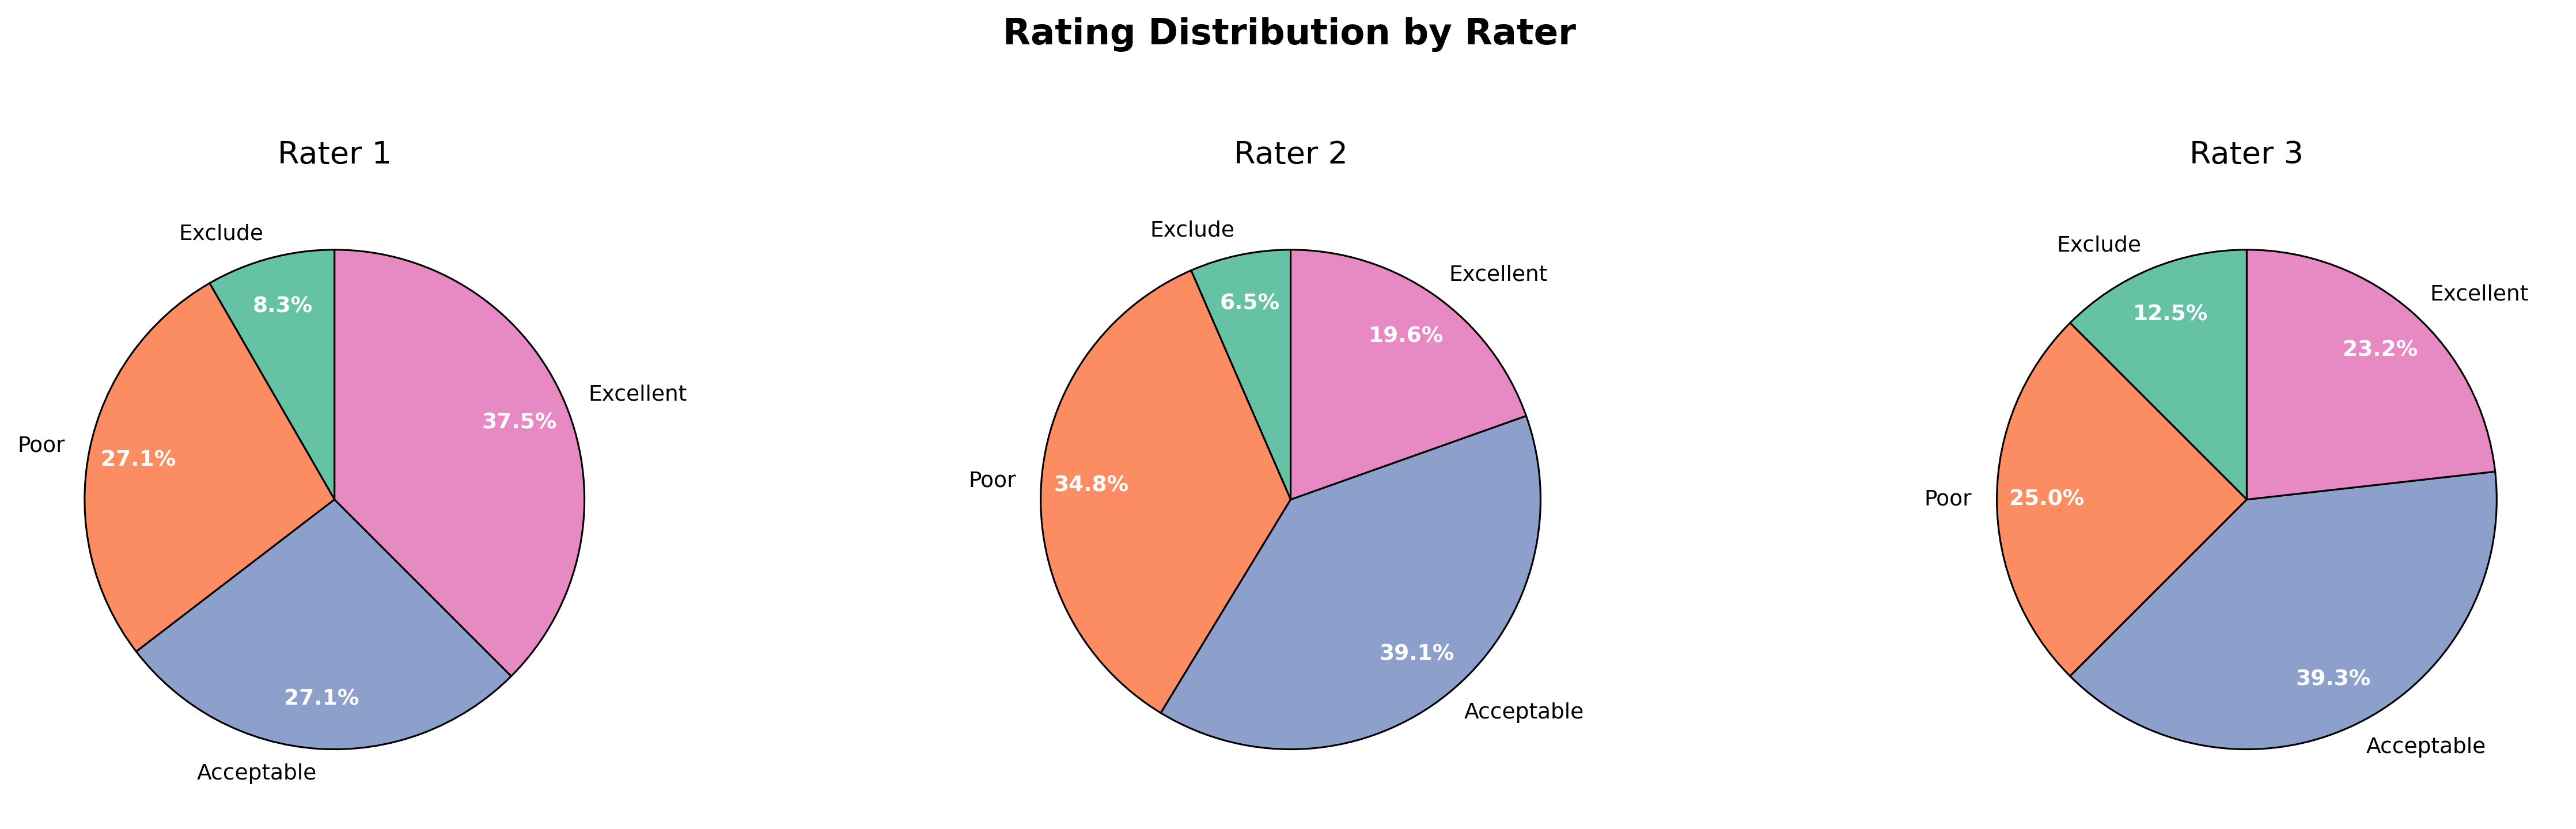
\includegraphics[width=1\linewidth]{Report/img/rating_by_rater_pie.png}
    \caption{Rating distribution by rater across 'Exclude', 'Poor', 'Acceptable', and 'Excellent' categories. Note the variations in how frequently each rater assigned images to the different quality categories. Figure from others degradation are in \ref{app:distribution}}
    \label{fig:rating_distribution_by_rater}
\end{figure}

As shown in Figure~\ref{fig:rating_distribution_by_rater}, analysis of image quality ratings reveals significant inter-rater variability across the four defined categories: “Exclude,” “Poor,” “Acceptable,” and “Excellent.” This demonstrates, first, the difficulty of manually classifying image quality. This already represents a challenge for the project, as having a benchmark rating is essential for the project. A key observation is the varying rigor between raters. Rater 3, for example, displayed the strictest rating trends, classifying 12.5\% of images as “Exclude.” This figure is significantly higher than that of Rater 1 (8.3\%) and is nearly double the proportion designated by Rater 2 (6.5\%) for the same critical category. Conversely, Rater 1 showed the greatest tolerance for good quality images, rating 37.5\% of images as “Excellent,” compared to 19.6\% for Rater 2 and 23.2\% for Rater 3.

Overall, differences are discernible in how each reviewer interprets the quality assessment criteria. This variability may pose a challenge when training the model.

\subsubsection{Inter-Rater Reliability Assessment Methodology}
\label{sssec:irr_methodology}
To quantitatively measure the consistency between the three evaluators, we performed three statistical measures for each image quality metric evaluated:
\begin{itemize}
    \item \textbf{Intraclass Correlation Coefficient (ICC):} Specifically, the ICC(A,k) coefficient is used to assess the agreement of the average measurements of $k=3$ raters. This coefficient indicates the consistency with which raters rated the images on a continuous scale (0-4). Values close to 1 indicate higher agreement, with an ICC coefficient > 0.75 generally considered good to excellent reliability.
    \item \textbf{Percentage Agreement:} For the 'Eyes Open Status', a simple percentage agreement was also determined, representing how often all three raters assigned the exact same category.
    \item \textbf{Correlation matrix} Indicate the correlation between each rating evaluated by the evaluators. This allows you to know if an artifact has a good correlation with the overall rating or if certain artifacts are correlated with each other.
\end{itemize}
\subsubsection{Inter-Rater Reliability Assessment Results}
\label{sssec:irr_results}
The results of this reliability analysis are summarized in table ~\ref{tab:irr_results_actual} and illustrated in more detail by the correlation matrices in figures \ref{fig:cm_all_raters_rc}. The different ratings are defined as, "rating 1" is the rating on the optical parts of the eye (globe and lens), "rating 2" is the rating on the non-optical parts of the eye (muscle, optic nerve, fat) and "rating" is the overall rating of the image averaged over all ratings.

% \begin{table}[htbp]
% \centering
% \caption{Inter-Rater Reliability Metrics for Image Quality Assessments}
% \label{tab:irr_results_actual}
% \resizebox{\textwidth}{!}{
% \begin{tabular}{lcccc}
% \toprule
% \textbf{Metric} & \textbf{ICC(A,k)} & \textbf{ICC CI95\% Low} & \textbf{ICC CI95\% High} & \textbf{\% Agreement} \\
% \midrule
% rating          & -0.149   & -1.490          & 0.520           & -            \\
% rating1         & 0.144    & -0.820          & 0.640           & -            \\
% rating2         & -0.293   & -1.800          & 0.460           & -            \\
% blur            & -0.289   & -1.510          & 0.430           & -            \\
% noise           & -0.404   & -1.960          & 0.400           & -            \\
% motion          & 0.136    & -0.800          & 0.630           & -            \\
% bgair           & -0.328   & -2.020          & 0.450           & -            \\
% Eyes Open Status& -        & -               & -               & 40.000       \\
% \bottomrule
% \end{tabular}
% } 
% \end{table}
\begin{table}[htbp]
\centering
\caption{Inter-Rater Reliability Metrics for Image Quality Assessments}
\label{tab:irr_results_actual}
\resizebox{\textwidth}{!}{
\begin{tabular}{lcccc}
\toprule
\textbf{Metric} & \textbf{ICC(A,k)} & \textbf{ICC CI95\% Low} & \textbf{ICC CI95\% High} & \textbf{\% Agreement} \\
\midrule
rating & 0.854 & 0.780 & 0.900 & - \\
rating1 & 0.889 & 0.830 & 0.930 & -0.005 \\
rating2 & 0.775 & 0.660 & 0.850 & - \\
blur & 0.580 & 0.370 & 0.730 & -0.065 \\
noise & 0.562 & 0.350 & 0.710 & 0.025 \\
motion & 0.705 & 0.560 & 0.810 & 0.206 \\
bgair & 0.588 & 0.380 & 0.730 & 0.255 \\
Eyes Open Status & - & - & - & 83.820 \\
\bottomrule
\end{tabular}
}
\end{table}
%\paragraph{Interpretation of Continuous Ratings (ICC)}
% The intraclass correlation coefficient values for overall quality assessments (“rating”, “rating1”, “rating2”) and specific artifact scores (“blur”, “noise”, “motion”, “bgair”) are consistently low, often negative. For example, “rating” yielded an ICC(A,k) of -0.149 (95\% CI: [-1.490, 0.520]), and “noise” an ICC of -0.404 (95\% CI: [-1.960, 0.400]). According to common interpretation guidelines (\cite{koo_guideline_2016}), ICC values below 0.5 indicate low reliability. The resulting ICC values, many of which are negative or close to zero, and their wide 95\% confidence intervals, suggest a lack of consistency among raters when assessing these measures on a continuous scale.
% For the "Eyes Open State" measure, the percentage agreement is 40.00\%. This relatively low agreement further highlights the difficulty of obtaining consistent manual assessments.

% Overall, the inter-rater reliability analysis consistently indicates low consistency between the three raters for the majority of image quality indicators assessed. This low reliability suggests the difficulty of systematically applying the evaluation criteria and the difficulty of having an accurate ground truth.

The results of the inter-rater reliability analysis, presented in Table 1, show variability in the consistency of assessments between the three raters for different image quality measures.
According to the interpretation guidelines (\cite{koo_guideline_2016}), ICC values between 0.5 and 0.75 indicate moderate reliability, while those above 0.75 indicate excellent reliability.

For overall quality assessments, such as "rating," "rating1," and "rating2," the intraclass correlation coefficients (ICC(A,k)) are relatively high, indicating good reliability. For example, "rating" yielded an ICC(A,k) of 0.854 (95\% CI: [0.780, 0.900]) and "rating1" an ICC(A,k) of 0.889 (95\% CI: [0.830, 0.930]). These values, significantly higher than 0.75, are therefore considered excellent inter-rater consistency for these overall scores.

Regarding scores for specific artifacts such as "blur," "noise," and "bgair," the ICC(A,k) values are moderate. "Blur" has an ICC(A,k) of 0.580 (95\% CI: [0.370, 0.730]), "noise" of 0.562 (95\% CI: [0.350, 0.710]), "motion" of 0.705 (95\% CI: [0.560, 0.810]), and "bgair" of 0.588 (95\% CI: [0.380, 0.730]). These values show that it is more difficult to annotate artifacts than to rate the overall image or a specific class.

Finally, for the "Eyes Open Status" metric, the percentage agreement is 83.82\%. This high percentage of agreement for a binary or categorical variable is a strong indicator of consistency for this specific assessment.

In summary, the inter-rater reliability analysis reveals that raters exhibit good to excellent consistency for overall image quality assessments (“grade”, “grade1”, “grade2”). However, reliability is more moderate for specific artifacts (“blur”, “noise”, “bgair”) and reasonably good for “motion”.

\begin{figure}[htbp]
    \centering
    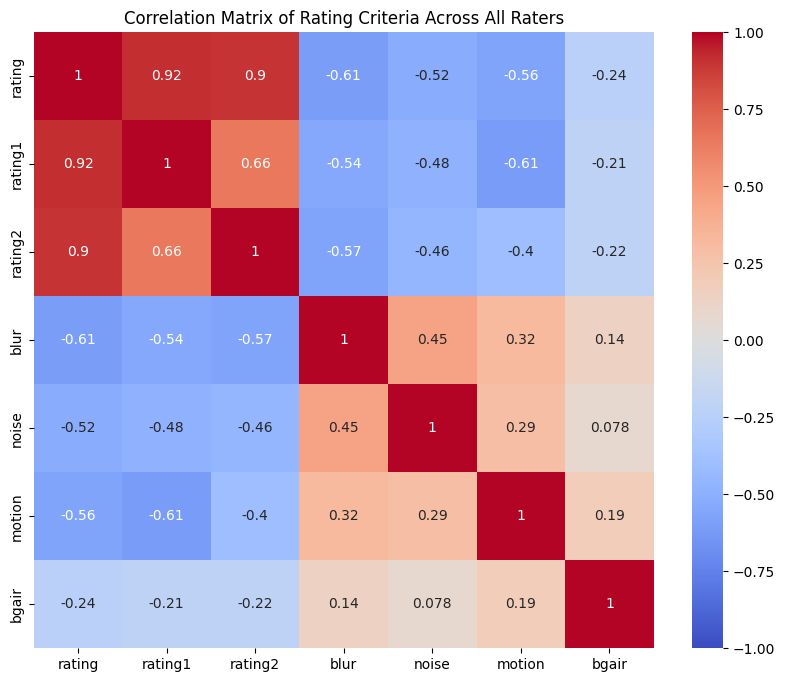
\includegraphics[width=0.5\textwidth]{Report/img/CM_of_all_raters_RC.png}
    \caption{Correlation Matrix of rating criteria across all raters}
    \label{fig:cm_all_raters_rc}
\end{figure}

Overall, there is no strong correlation between artifacts. The artifacts seem to contain unique features, which is important information for the rest of the project. Note that noise and blur have a correlation of 0.45, this suggests that severely blurred images are often perceived as noisy, which could reflect common degradation pathways or the difficulty distinguishing these artifacts during human evaluation.
Blur shows the strongest correlation with our overall image quality score, with a coefficient of -0.61. This indicates a strong inverse relationship: as perceived blur increases, the overall image quality score tends to decrease significantly.


\subsection{Which Image Artifacts Most Impact Human Quality Judgments?}
\label{sec:artifact_impact_lmm}

After assessing the reliability (and limitations) of manual assessments, the next objective is to identify the specific visual artifacts with the most significant independent influence on overall image quality assessments. This is essential for prioritizing IQMs sensitive to the most significant image degradations. To achieve this, we used a linear mixed-effects model (LMM). This statistical approach allows us to model the relationship between the overall quality score and the scores of individual artifacts.

\begin{table}[htbp]
    \centering
    \caption{Simplified Linear Mixed-Effects Model Results (Dependent Variable: rating)}
    \label{tab:lmm_results_from_doc}
    \begin{tabular}{>{\raggedright\arraybackslash}p{2cm}rrrrrr}
    \toprule
        \multicolumn{7}{c}{\textbf{Dependent Variable: rating}} \\
        \textbf{Effect}      & \textbf{Coef.}  & \textbf{Std.Err.} & \textbf{z}       & \textbf{P$>$$|$z$|$} & \textbf{[0.025} & \textbf{0.975]} \\
    \midrule
        Intercept   & 3.081  & 0.106    & 29.159 & 0.000       & 2.874  & 3.288  \\
        blur        & -0.288 & 0.064    & -4.522 & 0.000       & -0.412 & -0.163 \\
        noise       & -0.254 & 0.070    & -3.645 & 0.000       & -0.391 & -0.118 \\
        motion      & -0.204 & 0.061    & -3.313 & 0.001       & -0.324 & -0.083 \\
        bgair       & -0.122 & 0.072    & -1.701 & 0.089       & -0.263 & 0.019  \\
    \midrule
        \multicolumn{7}{l}{\textbf{Random Effect Variance:}} \\
        sub Var     & 0.075  & \multicolumn{2}{l}{(SE: 0.098)} &             &        &        \\
    \midrule
        \multicolumn{7}{l}{\textbf{Model Fit:}} \\
        \multicolumn{7}{p{\dimexpr\linewidth-2\tabcolsep\relax}}{No. Obs: 151, No. Groups: 83, Scale (Residual Var): 0.1809, Log-Likelihood: -115.38} \\
        \multicolumn{7}{l}{Converged: Yes, Method: REML} \\
    \bottomrule
    \end{tabular}
\end{table}

\textbf{Key Findings from the LMM:}

The LMM results (summarized in Table~\ref{tab:lmm_results_from_doc}) pinpoint the artifacts that statistically significantly degraded the perceived image quality:

\begin{itemize}
    \item \textbf{Blur:} Show the \textbf{strongest negative impact}. For each one-unit increase in perceived blur, the overall quality rating decreased by approximately 0.288 ($p < 0.001$).
    \item \textbf{Noise:} Also a significant factor, with each unit increase in noise lowering the quality rating by about 0.254 ($p < 0.001$).
    \item \textbf{Motion:} Have a significant negative effect, reducing the quality rating by roughly 0.204 ($p = 0.001$).
    \item \textbf{Background Artifacts ('bgair'):} In this model, once blur, noise, and motion were accounted for, 'bgair' did not show a statistically significant independent effect on the overall quality rating ($p = 0.089$). While not statistically significant in this specific model, visual reports and qualitative analysis still suggested `bgair` as a relevant factor.
\end{itemize}

\textbf{Implications for IQM Selection:}

The LMM result provides clear guidelines for the IQM strategy. Artifacts, blur, noise, and motion are the main culprits of image quality degradation from the evaluators' perspective, with blur being the most significant. Therefore, IQMs must include robust metrics capable of detecting and quantifying these three artifacts. Background artifacts were not significant for the quality degradation but we will see later (Section~\ref{sssec:initial_rater_distribution}) which will still be useful


\section{Visual Analysis of Image Quality Classes}
\label{sec:visual_analysis_iq_classes}

In order to refine the selection of IQMs and to complete the statistical results, we carried out a qualitative visual evaluation on images manually classified into three categories: "Excluded", "Poor" composed of "poor" and "acceptable" and "Excellent". This observation is carried out on the segmentation of 3D eye images of a pre-trained nnUnet v1 model. It aims to show the difficulty that the model has in identifying the different segmentation classes such as the globe, the lens, the muscles, the optic nerve, the fat.

\subsection{Excluded Images: Severe Degradation}
\label{sec:excluded_images}
Excluded images are usually characterized by a severe degradation in overall image quality. These characteristics make them unusable for analysis and therefore must be excluded. Here are different images showing the degradations
\begin{figure}[htbp]
    \centering
    \begin{subfigure}[b]{0.35\textwidth} 
        \centering
        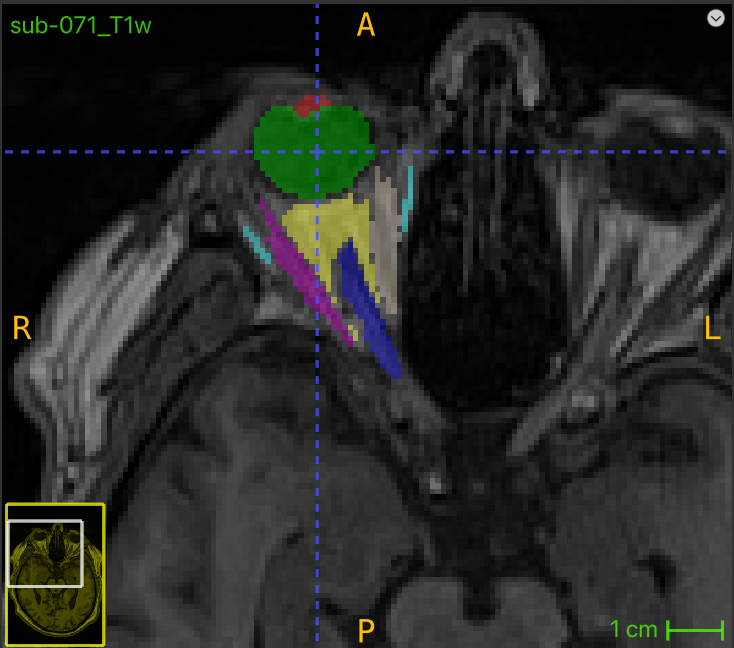
\includegraphics[width=\linewidth]{Report/img/sub-071_T1w.png}
        \caption{T1w - Subject 071}
        \label{subfig:071_T1w}
    \end{subfigure}
    \hspace{0.02\textwidth}
    \begin{subfigure}[b]{0.375\textwidth}
        \centering
        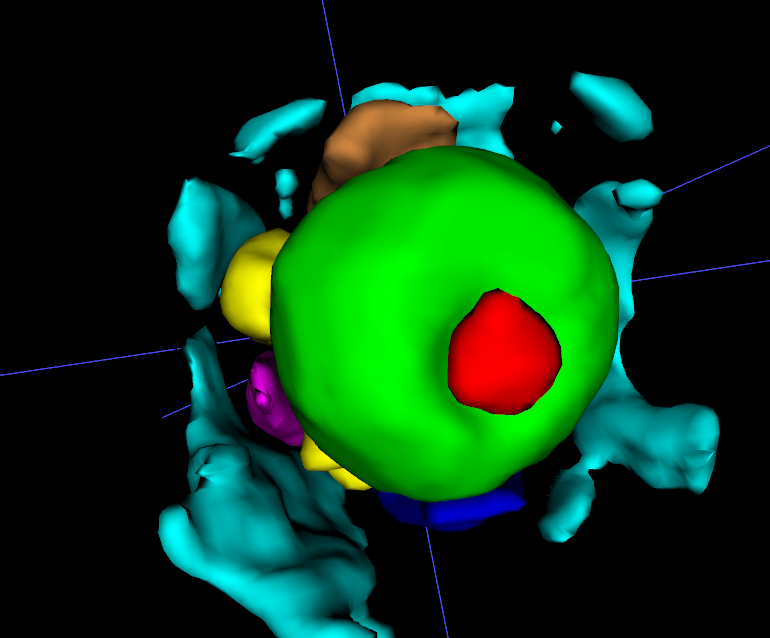
\includegraphics[width=\linewidth]{Report/img/sub-071_T1w_3D.png}
        \caption{T1w\_3D - Subject 071}
        \label{subfig:071_T1w_3D}
    \end{subfigure}

    \vspace{2mm} % Vertical space between rows

    \begin{subfigure}[b]{0.35\textwidth} 
        \centering
        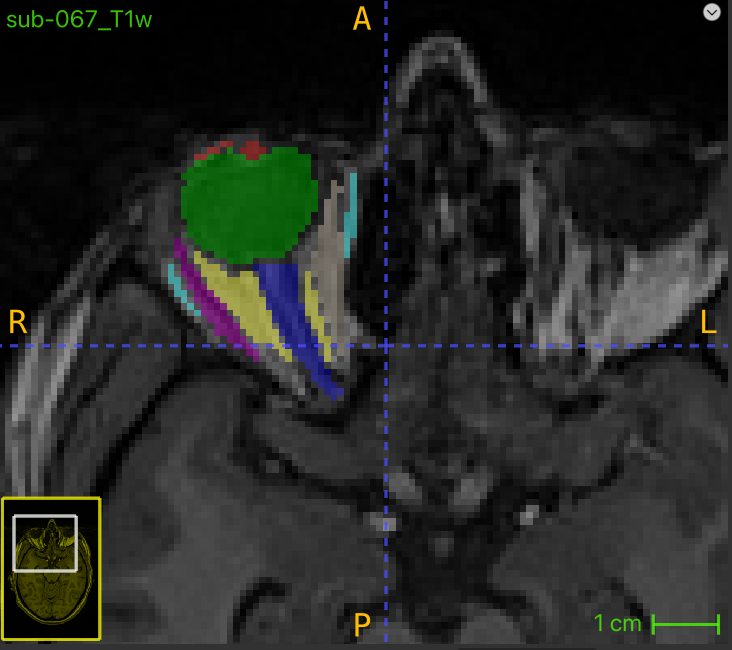
\includegraphics[width=\linewidth]{Report/img/sub-067_T1w.png}
        \caption{T1w - Subject 067}
        \label{subfig:067_T1w}
    \end{subfigure}
    \hspace{0.02\textwidth} 
    \begin{subfigure}[b]{0.375\textwidth} 
        \centering
        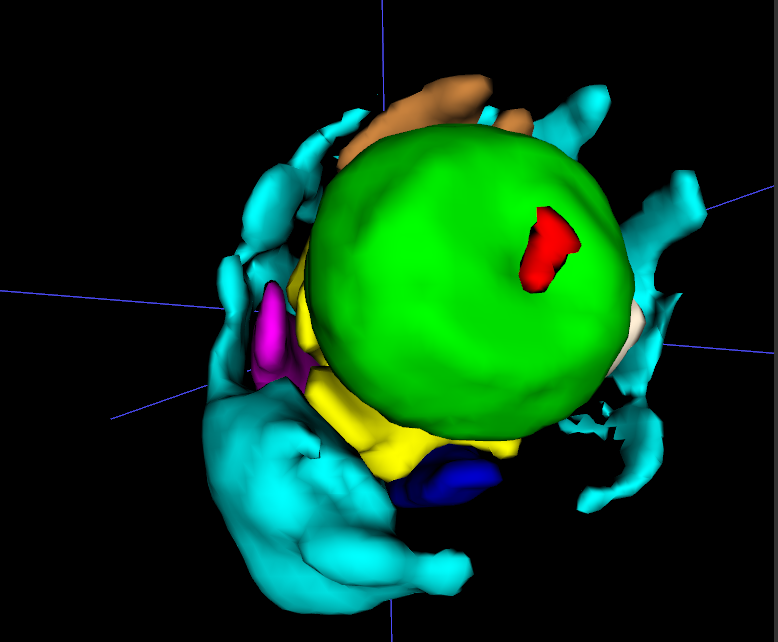
\includegraphics[width=\linewidth]{Report/img/sub-067_T1w_3D.png}
        \caption{T1w\_3D - Subject 067}
        \label{subfig:067_T1w_3D}
    \end{subfigure}
    \caption{Comparison between T1w (left column) and T1w\_3D (right column) images categorized as 'Excluded' quality. These examples demonstrate severe lens segmentation issues, geometric distortions, and general image degradation.}
    \label{fig:excluded_images}
\end{figure}

\subsubsection{Observation}
In the segmented excluded images, severe deficiencies are consistently observed. The lenses are poorly segmented, often deviating significantly from their characteristic ellipsoidal shape. Similarly, the globe segmentation exhibits notable surface imperfections. Furthermore, muscle segmentation frequently contains aberrations, with multiple unrelated pieces being segmented, leading to overall poor quality.

\subsection{Poor Quality Images: Noticeable Imperfections}
\label{sec:bad_quality_images}
Images in the Poor Quality category (poor and acceptable class) are not necessarily unusable, but they do have notable imperfections that distinguish them from excellent quality. That said, they are not as severely compromised as Excluded images, which still makes them usable for analysis. Here are some images of the resulting degradation
\begin{figure}[htbp]
    \centering
    \begin{subfigure}[b]{0.35\textwidth}
        \centering
        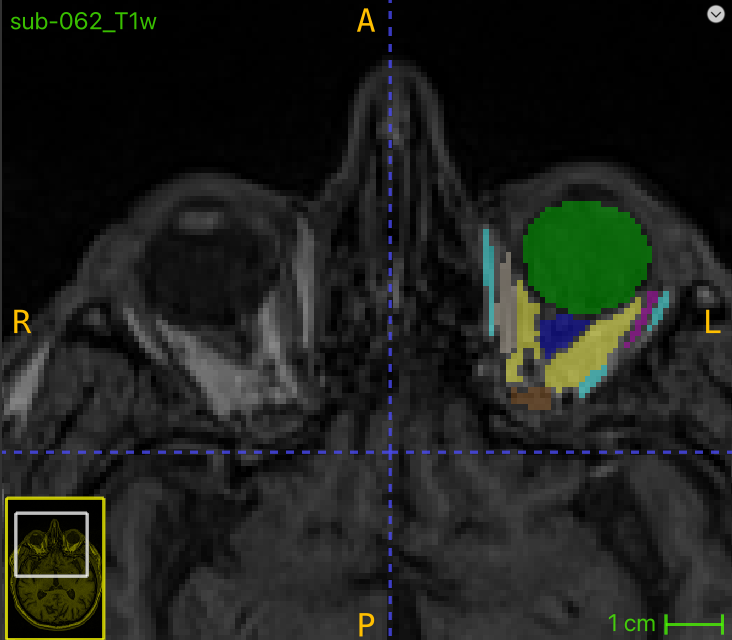
\includegraphics[width=\linewidth]{Report/img/sub-062_T1w.png}
        \caption{T1w - Subject 062}
        \label{subfig:062_T1w}
    \end{subfigure}
    \hspace{0.02\textwidth}
    \begin{subfigure}[b]{0.375\textwidth} 
        \centering
        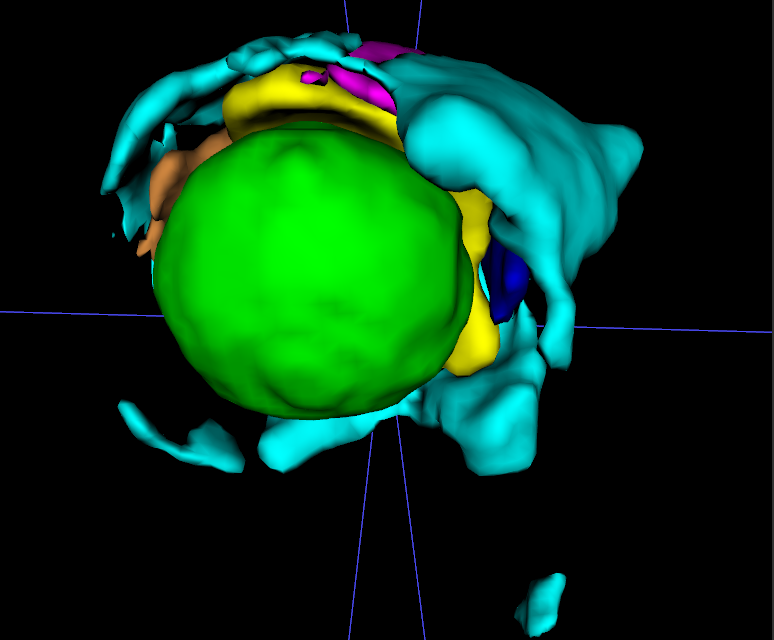
\includegraphics[width=\linewidth]{Report/img/sub-062_T1w_3D.png}
        \caption{T1w\_3D - Subject 062}
        \label{subfig:062_T1w_3D}
    \end{subfigure}

    \vspace{2mm} 

    % Second row of images
    \begin{subfigure}[b]{0.35\textwidth} 
        \centering
        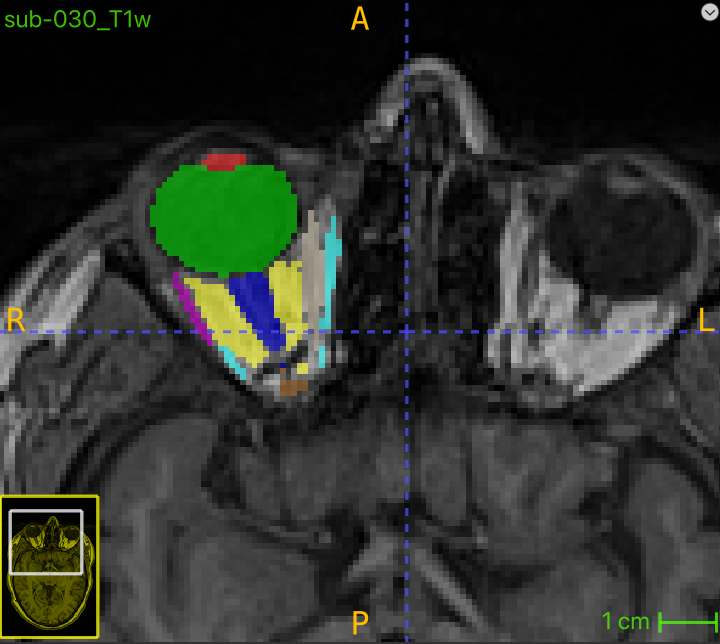
\includegraphics[width=\linewidth]{Report/img/sub-030_T1w.png}
        \caption{T1w - Subject 030}
        \label{subfig:030_T1w}
    \end{subfigure}
    \hspace{0.02\textwidth} 
    \begin{subfigure}[b]{0.375\textwidth} 
        \centering
        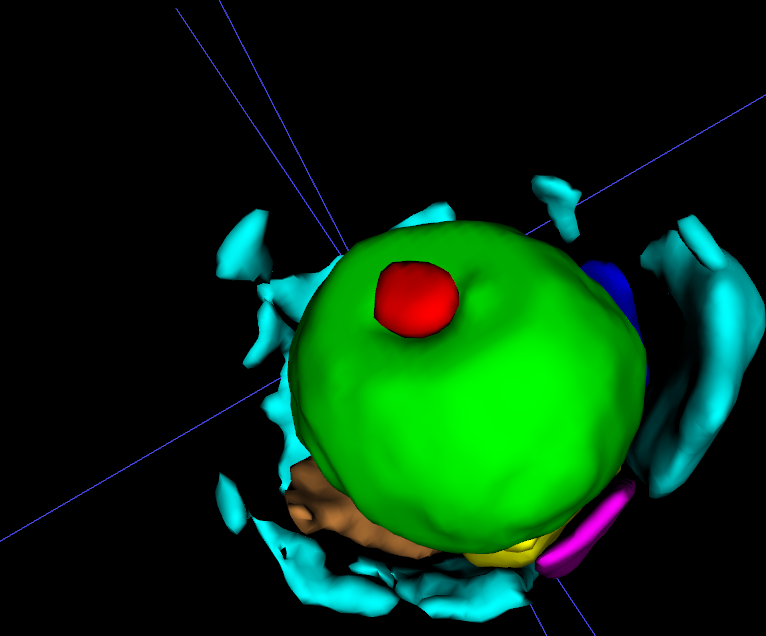
\includegraphics[width=\linewidth]{Report/img/sub-030_T1w_3D.png}
        \caption{T1w\_3D - Subject 030}
        \label{subfig:030_T1w_3D}
    \end{subfigure}
    \caption{Comparison between T1w (left column) and T1w\_3D (right column) images categorized as 'Poor' quality. These examples show noticeable but not severe blur and minor segmentation imperfections.}
    \label{fig:bad_quality_images}
\end{figure}

\subsubsection{Observation}
The 'Poor Quality' category, while also exhibiting aberrations in lens, globe, and muscle segmentations, differs from the 'Excluded' category in that these imperfections are typically isolated and less severe. Consequently, images in this category are generally still considered usable
\newpage

\subsection{Excellent Quality Images: High Fidelity}
\label{sec:excellent_quality_images}
Excellent quality images represent the ideal standard. They are characterized by high fidelity and clarity, making them optimal for further analysis. They do not present any severe degradation in any of the eye segmentation parts. Here are some of the results obtained

\begin{figure}[htbp]
    \centering
    % First row of images
    \begin{subfigure}[b]{0.35\textwidth} % Adjust subfigure width to fit content
        \centering
        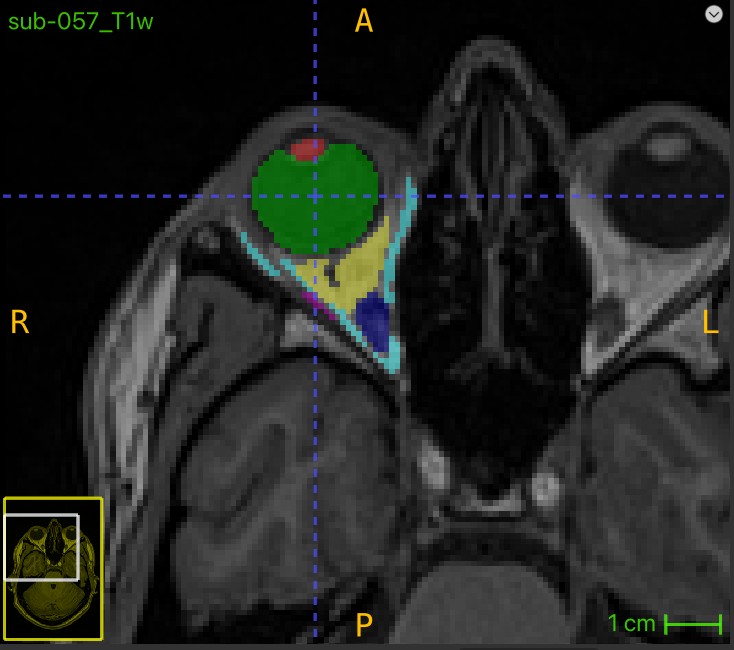
\includegraphics[width=\linewidth]{Report/img/sub-057_T1w.png}
        \caption{T1w - Subject 057}
        \label{subfig:057_T1w}
    \end{subfigure}
    \hspace{0.02\textwidth} % Small horizontal space between images
    \begin{subfigure}[b]{0.375\textwidth} % Adjust subfigure width
        \centering
        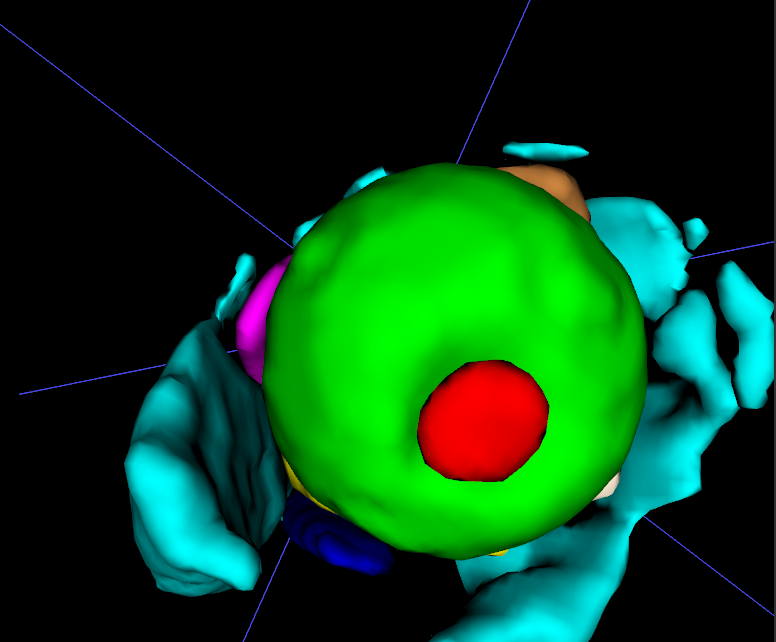
\includegraphics[width=\linewidth]{Report/img/sub-057_T1w_3D.png}
        \caption{T1w\_3D - Subject 057}
        \label{subfig:057_T1w_3D}
    \end{subfigure}

    \vspace{2mm} % Vertical space between rows

    % Second row of images
    \begin{subfigure}[b]{0.35\textwidth} % Adjust subfigure width
        \centering
        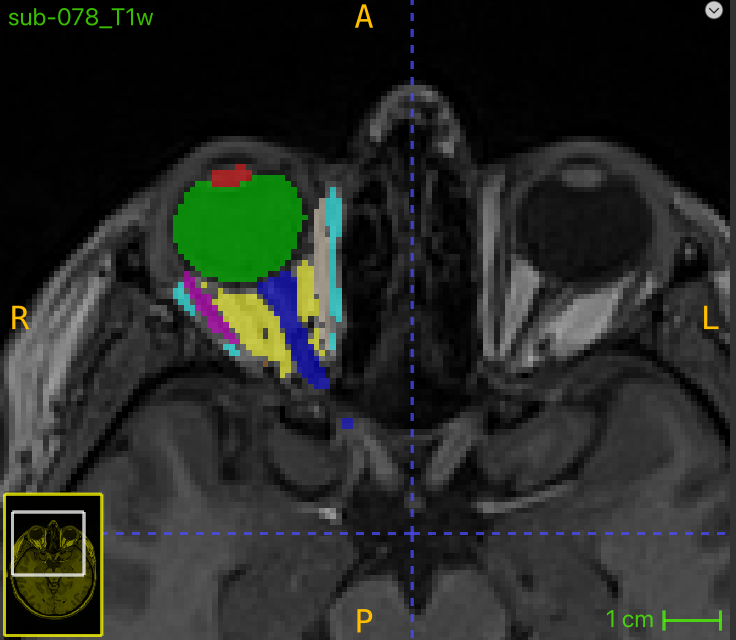
\includegraphics[width=\linewidth]{Report/img/sub-078_T1w.png}
        \caption{T1w - Subject 078}
        \label{subfig:078_T1w}
    \end{subfigure}
    \hspace{0.02\textwidth} % Small horizontal space between images
    \begin{subfigure}[b]{0.375\textwidth} % Adjust subfigure width
        \centering
        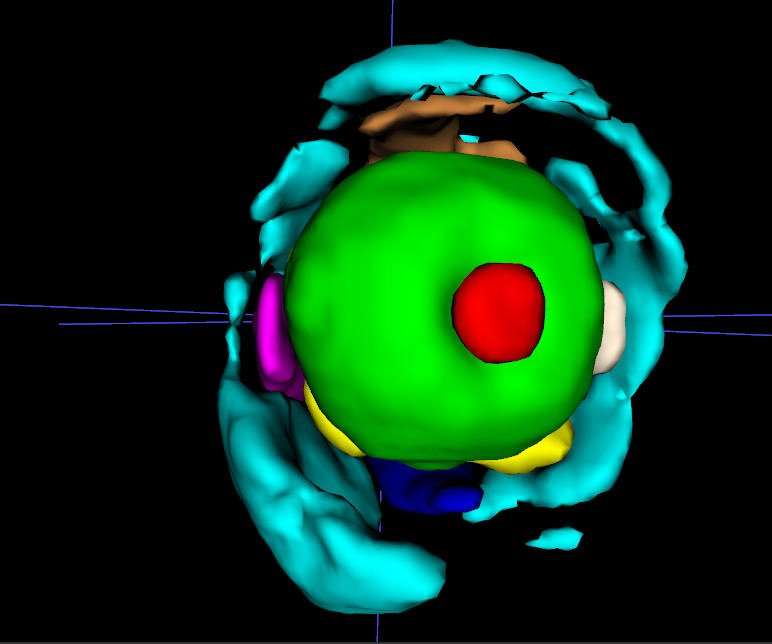
\includegraphics[width=\linewidth]{Report/img/sub-078_T1w_3D.png}
        \caption{T1w\_3D - Subject 078}
        \label{subfig:078_T1w_3D}
    \end{subfigure}
    \caption{Comparison between T1w (left column) and T1w\_3D (right column) images categorized as 'Excellent' quality. These examples showcase clear anatomical delineation, accurate segmentations, and minimal artifacts.}
    \label{fig:excellent_quality_images}
\end{figure}

\subsubsection{Observation}
Images categorized within this class are distinguished by segmentations of exceptionally high quality. Their surfaces are precisely delineated, and the morphology of the various ocular components faithfully adheres to established human anatomy. This class is notably characterized by the near-complete absence of image deterioration
\subsection{Observations Summary for IQM Selection}
\label{sec:iqm_selection_summary}
In the segmented excluded images, the lenses exhibit distinct segmentation problems. These lenses often display discontinuous or aberrant shapes that do not correlate with the true anatomical form of a human lens, underscoring the importance of incorporating lens-segmentation-based IQMs. Regarding the Globe, it is observable that globes in excellent quality images possess a notably smoother surface compared to those found in excluded or poor-quality images. This distinction highlights the importance of basing IQMs on this segmentation class as well. For the other classes, no noticeable differences are consistently apparent between excluded images and excellent quality ones. This observation is attributed to the inherent complex morphology of these classes, which impedes the easy visual identification of segmentation discrepancies.